\chapter{Welke stappen zijn er nodig om een traditionele website om te vormen tot een PWA}
\label{ch:TransformerenNaarEenPWA}



Voor sommige webapplicaties is het een grote meerwaarde om geïnstalleerd te kunnen worden  en offline bruikbaar te zijn op het toestel van de gebruiker.\autocite{Mozilla2020c} Eenvoudige applicaties die geen gebruik maken van een backend verzoeken kunnen op deze manier volledig functioneel zijn zonder internetconnectie. 
Aan de hand van dit voorbeeld zal de onderzoeksvraag “Welke stappen zijn nodig om een traditionele website om te vormen tot een PWA?” beantwoord worden.

\section{De applicatie}

	Darts is een spel dat gespeeld wordt met drie pijltjes per persoon en een dartbord. De plaats waar het pijltje landt op het bord bepaalt de score van de worp, dit kan variëren van 0 tot 60. De speler die het eerst een score van 501 bij elkaar gooit is de winnaar. Deze score’s optellen en bijhouden wordt al snel ingewikkeld. Darts is een spel dat vaak gespeeld wordt in een bar, spelers willen dus niet geconcentreerd moeten rekenen. Spelers zullen dus vaak op zoek gaan naar hulpmiddelen, dit kan een combinatie zijn van pen en papier met een rekenmachine, een alternatief is een native applicatie die dit doet voor hen. Bij deze applicatie zal deze service aangeboden worden als een PWA, hij kan dus gebruikt worden in de browser, de applicatie kan ook gedownload worden.

\section{Analyse}

	Er werden user-stories opgesteld zodat de requirements van de applicatie duidelijk werden.  
	
	\begin{itemize}
		 \item 	Als een speler wil ik de score van een spel kunnen bijhouden zonder een applicatie te downloaden zodat mijn gsm niet vol komt met applicatie.
		 \item 	Als een speler wil ik de score van een dartspel op mijn smartphone kunnen bijhouden zodat ik altijd en overal kan spelen.
		 \item 	Als een speler wil ik de score van een dartspel bijhouden zonder een internetverbinding te hebben zodat ik niet afhankelijk ben van een eventuele wifi of een netwerkverbinding.
		 \item 	Als een groep vrienden willen we een dartspel kunnen starten en de score kunnen bijhouden voor een variabel aantal personen zodat we snel kunnen spelen.
		 \item Als een ontwikkelaar wil ik aan alle voorwaarden van de ligthouse audit op vlak van PWA's voldoen zodat de applicatie volledig geoptimaliseerd is.
	\end{itemize}	
	
	
	%TODO: wat zijn de niet functionele requirements? de audit misschien hier al vermelden


\section{Implementatie}

	De applicatie werd eerst ontworpen aan de hand van figma, dit is een tool die gebruikt wordt om designs en prototypes te maken. De applicatie zal drie schermen hebben: een die het aantal speler vraagt, een die de spelersnamen vraagt en een scherm waar het spel kan bijgehouden worden. 
	Voor de ontwikkeling van de applicatie werd de javascript library React.js gekozen.
	
	
	\begin{figure}[H]
		\centering
		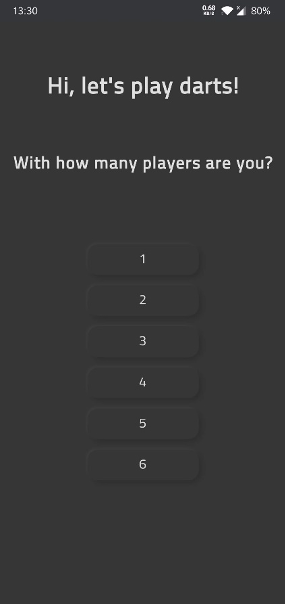
\includegraphics[width=35mm]{./img/dart1.png}{}
		\caption{startscherm – vragen naar het aantal spelers}
	\end{figure}
	
	\begin{figure}[H]
		\centering
		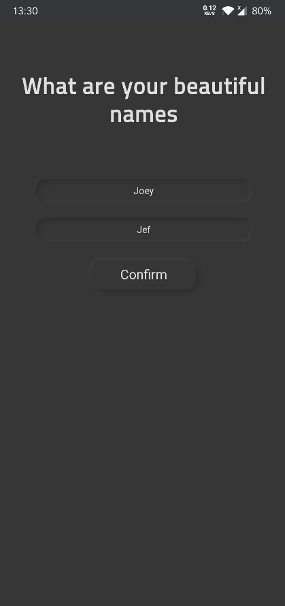
\includegraphics[width=35mm]{./img/dart2.png}{}
		\caption{vragen naar de namen van de spelers}
	\end{figure}
	
	\begin{figure}[H]
		\centering
		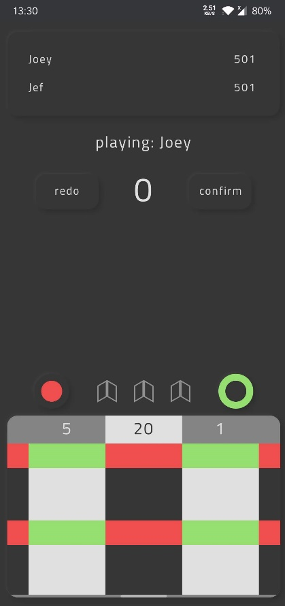
\includegraphics[width=35mm]{./img/dart3.png}{}
		\caption{het scherm waar de score geteld zal worden}
	\end{figure}
	


\section{A2HS}

	Een PWA is een applicatie die gebruik maakt van moderne webtechnologieën. Dit is geen meetbare definitie, voor dit onderzoek zullen een website optimaliseren tot deze een beforeinstallprompt kan activeren. Dit wil zeggen dat de website toegevoegd kan worden op het toestel van de gebruiker.

	\subsection{HTTPS}

		Een van de drie vereisten om een applicatie te kunnen toevoegen aan het startscherm is dat er een https-connectie moet zijn. Dit werd bekomen door de website te hosten op \href{https://www.netlify.com/}{ Netlify}. Dit is een online service die gratis hosting voor statische websites aanbiedt en hier kan ook een SSL-certificaat toegevoegd worden zodat er een HTTPS connectie tot stand komt.


	\subsection{App manifest}
\begin{lstlisting}
{
  "short_name": "Dart 501",
  "name": "Dart 501",
  "icons": [
   {
     "src": "/icons/android-icon-36x36.png",
     "sizes": "36x36",
     "type": "image/png",
     "density": "0.75"
   },
   {
     "src": "/icons/android-icon-48x48.png",
     "sizes": "48x48",
     "type": "image/png",
     "density": "1.0"
   },
   {
     "src": "/icons/android-icon-72x72.png",
     "sizes": "72x72",
     "type": "image/png",
     "density": "1.5"
   },
   {
     "src": "/icons/android-icon-96x96.png",
     "sizes": "96x96",
     "type": "image/png",
     "density": "2.0"
   },
   {
     "src": "/icons/android-icon-144x144.png",
     "sizes": "144x144",
     "type": "image/png",
     "density": "3.0"
   },
   {
     "src": "/icons/android-icon-192x192.png",
     "sizes": "192x192",
     "type": "image/png",
     "density": "4.0"
   },
   {
     "src": "logo512.png",
     "type": "image/png",
     "sizes": "512x512"
   }
  ],
  "start_url": ".",
  "display": "standalone",
  "theme_color": "#95df71",
  "background_color": "#363636"
}
	
\end{lstlisting}
		
		De naam en de verkorte naam (naam die op startscherm getoond zal worden) worden als eerste vastgelegd. Deze zijn gelijk omdat de volledige naam al kort genoeg is. Het maximumaantal karakters voor 'short\_name' is 12.
 
		
		Vervolgens worden alle iconen voor de verschillende platformen bepaald. Dit deel van het manifest en de bestanden waarnaar het refereert kunnen gegenereerd worden met een online tool \href{https://appicon.co}{appicon.co}
		
		Vervolgens wordt het gedrag en het uitzicht van de applicatie. Er wordt ingesteld dat de applicatie start op het scherm waar het aantal spelers geselecteerd kan worden, er wordt ook bepaald dat de applicatie het volledige scherm in beslag moet nemen.
		
		Ook het kleurenschema wordt bepaald, deze kleuren worden gebruikt bij het startscherm en bepalen ook de kleur van de statusbalk van het toestel. 
		
		Er moet een link gemaakt worden van de html-bestanden naar dit manifest bestand. Dit gebeurt binnen de head tags van de index.html file
		
\begin{lstlisting}
	<link rel="manifest" href="%PUBLIC_URL%/manifest.json" />
\end{lstlisting}
		
		
	\subsection{Service worker}
		
		Als een react applicatie gecreëert wordt met het 'create-react-app') commando wordt er standaard een basis service worker aangemaakt. Standaard wordt deze niet gebruikt, om dit te veranderen moet de regsiter methode van de service worker aangeroepen worden in het index.js bestand.
		
\begin{lstlisting}
		serviceWorker.register();
\end{lstlisting}
		
		Deze service worker zorgt ervoor dat alle statische bestanden offline beschikbaar gemaakt worden en dat de gebruiker op een Android toestel de vraag krijgt om deze applicatie aan het startscherm toe te voegen.
		
		Voor deze applicatie zijn biedt deze service worker genoeg functionaliteit.
		

\section{Controle}

	Aan de hand van een lighthouse audit kan er gecontroleerd worden als alles werkt zoals verwacht.
	
	\begin{figure}[H]
		\centering
		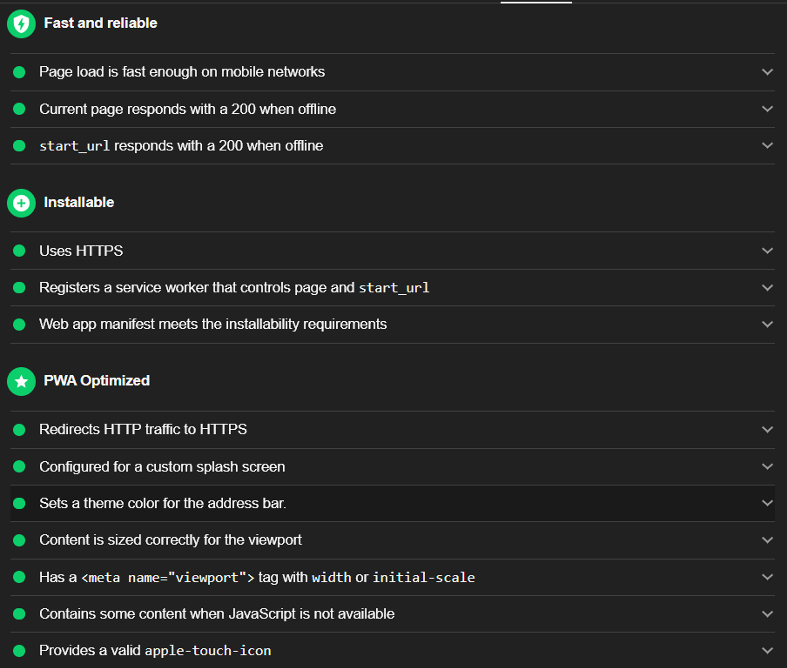
\includegraphics{./img/lighthouse_dart.png}{}
		\caption{lighthouse audit van de website}
	\end{figure}

	Onder de sectie ‘installable’ kunnen we zien dat de applicatie inderdaad een https-connectie heeft, dat er een service worker is en dat er een manifest aanwezig is.
	
	
	
\section{Conclusie}

	We kunnen concluderen dat een traditionele website snel kan omgevormd worden tot een PWA die geïnstalleerd kan worden op het startscherm van de gebruiker. 
	
	Zoals eerder aangehaald met een website aan volgende 3 zaken voldoen om geïnstalleerd te kunnen worden
	\begin{itemize}
		\item Een HTTPS-connectie hebben
		\item Een app manifest hebben
		\item Een service worker registreren
	\end{itemize}	
	
	Een HTTPS-connectie opzetten gebeurt bij verschillenden hosting services automatisch en gratis. Dit is dus eenvoudig op te zetten.
	
	De app manifest is een json-bestand die de eigenschappen van de applicatie beschrijft. Door gebruikt te maken van bepaalde tools kan dit ook snel gecreëerd worden.
	
	Als een webapplicatie ontwikkeld wordt met React.js kan ook een serviceworker eenvoudig geregistreerd worden. Er moet slecht één methode aangeroepen worden.
